\documentclass{article}
\usepackage[utf8]{inputenc}
\usepackage{graphicx}
\usepackage{float}
\usepackage{epsfig}
\usepackage{blindtext}
\usepackage{graphicx}
\usepackage[T1]{fontenc}
\usepackage{amsmath}

\title{MATH 444 Final Project}
\author{Connor Wolfe}
\date{May 2017}

\begin{document}

\maketitle

\section*{Introduction}
This assignment develops skills in building classification trees and then optimally pruning the tree to yield the most accurate classification.  We will first introduce the ideas and algorithms behind classification trees and how to prune them.  Next we will demonstrate findings on classifying the 'Irisdata.mat' set and the 'GlassData.mat' set.

\subsection*{Data Sets}
The 'GlassData.mat' contains the data set X (9x214) and annotation vector I (1x214).  The 9-dimensional data is classified by its refractive index, and weight percent of Na, Mg, Al, Si, K, Ca, Ba, Fe.  The annotation vector stores the class of each data point $I \epsilon [1, 2, 3, 4, 5, 6]$.  

\subsection*{Data Storage}
We will use structs to represent the trees.  The structs are stored in array R and sorted by index.  They will have the following properties:
\begin{verbatim}
   R(j).I= list of data point indices included in the rectangle 
   R(j).p= Frequency of each class
   R(j).j= The dimension of the data that is optimal to split
   R(j).s=  Value to split the rectangle into two optimally classified children 
   R(j).left= Index of left child
   R(j).right= Index of right child
\end{verbatim}
It is clear that when a rectangle has no children, we assign R(j).left=NaN and R(j).right=NaN, R(j).s=NaN, and R(j).j=NaN.  

\subsection*{Helper Functions}
\subsubsection*{ClassDistr}
Function to determine the frequency of each class of a given rectangle, the percent it misclassifies, and the majority class\\
Input:  C=vector of classes of data\\
        I= index vector corresponding to indices of data in rectangle in I\\
Output: p= vector of frequencies of each class (note the sum of elements in p=1)\\
        c= majority class (all data in this rectangle will be classified as c)\\
        r=misclassification error (rate that we misclassify points in this rectangle)\\
\\
Implementation:
\begin{verbatim}
function [p, c, r]=ClassDistr(C,I)
    n=size(I,2);  %total number of elements in the rectangle
    c=mode(C(I)); %c is the mode of the classes of the elements in the rectangle
    classes=unique(C); %find the class values
    k=size(classes,2); %and the number of classes to iterate through
    p=zeros(1,k);  %the size of p must be the number of classes
    for i=1:k
        num_i=size(find(C(I)==classes(i)),2); %find number of elements in class i
        p(i)=num_i/n; %divide this by the total number of elements for the frequency
    end
    r=1-p(c); %the misclassification error is 1 minus the frequency of the majority class, 
    %since all other elements are misclassified as this majority class
end
\end{verbatim}
\subsubsection*{OptimalSplit}
Function to return the data dimension and value to split the rectangle at in order to optimally classify the data
\\Input:  I\_ind=index vector corresponding to indices of data in rectangle in I
        \\C=vector of classes of data
        \\X=Data matrix
\\Output: j=dimension of x to split on
        \\s=value of x to split above and below

\\Implementation:
\begin{verbatim}
We must iterate through all dimensions of X and find within each dimension, which value 
s value would yield the best split.  We will store split values for each dimension in 
vector m\_j which stores the optimal split value and the mismatch it yields for each 
dimension. In order to calculate the split value given a dimension j, we do the following:
(a) Find the unique values of the data and sort them in increasing order.  We can now 
observe that the only splits which make sense are those between the sorted X points.  
In matlab we write:
    [x_sort, j_sort] = sort(x, 'ascend');
(b) Store every reasonable split value in vector s, where it will store the median 
between X(i) and X(i+1): 
        s(i)=0.5 * (x_sort(i) + x_sort(i+1));
(c) Sort the data points about the split value to yield the indices of the points 
left and right of it, and the class values of these points. 
        I_left=I(find(X(j,I) <= s(i)));
        c_left=C(I_left);
The same implementation holds for the right side.

(d) Calculate the mean of the values to the left and to the right
        c1=(1/(length(c_left)))*sum(c_left);  
(e) Calculate the mismatch of all X as its variance from the mean of the rectangle 
we sort it in:
        m_s(i)=sum((c_left - c1).^2) + sum((c_right-c2).^2);
(f) Return the split that minimizes the mismatch for this dimension and add it 
to the m_j vector
    [m_val, ind]=min(m_s);
    m_j(:,j)=[m_val;s_star];
(g) Once we have calculated the split for each j, we again minimize the mismatch 
within j to find the best j and s values
    [~, j_opt] = min(m_j(1,:));
    s_opt=m_j(2, j_opt);
(h) return j_opt and s_opt


\end{verbatim}
\subsubsection*{MisclassCost}
Input:  R=rectangle to analyze\\
        n= total number of data points in the set\\
        C= classification vector\\
Output: m= misclassification cost of the rectangle weighted by its size\\
Implementation: \\
First, we calculate the r value for rectangle R with the ClassDistr function, named r\_r\\
Next, we calculate the weight of the node as the number of elements inside it divided by the total number of elements:\\
    v\_r=length(R.I)/n;\\
Last, m is simply the product of v\_r and r\_r\\
m=v\_r*r\_r;\\


\section*{Building Classification Trees}

\subsection*{Idea}
A classification tree, as represented in figure (1) is a set of divisions of data into increasingly small rectangles.  The rectangle edges are calculated using the OptimalSplit() function to be the points which will best separate the data into its constituent classes.  When a rectangle is divided, the data inside is separated into the two child rectangles, left and right, depending on if the data is less than or greater than the threshold point, respectively.  Each child rectangle is assigned a class value based on the majority vote of the elements which compose it, and all data points inside will be approximated to this majority vote class.  It is important than that the rectangles capture the data well so that when we classify using their majority, we do not misclassify too many points.  
\\I will now describe the procedure for generating a classification tree that terminates with all pure leaves.  This procedure will begin with the entire data set R(1), and will continue to divide it using OptimalSplit() until all leaves are pure.  This tree rooted at R(1) and ending with all pure leaves we will call $T_{max}$

\begin{figure}[H]
    \centerline
    {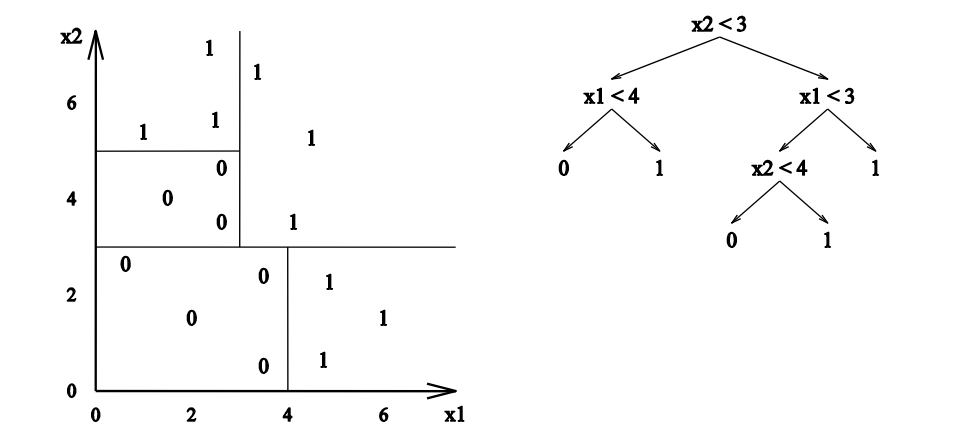
\includegraphics[width=12cm, height=5cm]{classification_tree_graphic.png}
    }
    \caption{\label{fig:my figure} An example of a classification tree for unrepresentative data.  We see the original tree $T_0$ divided into two smaller rectangles, points such that $x_2 <= 3$ or points such that $x_2 > 3$.  The graph continues to divide until all of the rectangles are of the same class (pure), yielding $T_{max}.$ }
\end{figure}

\subsection*{Algorithm}
1.  Initialize: Let R(1) be the rectangle containing all the data.  We set R(1).I=I
    \\Let PureNodes=[ ] be an empty vector that will store the pure nodes
    \\Let MixedNodes= [1] be a vector containing indices of the mixed nodes
    \\count=1;
\\2.  While length(MixedNodes)>0 %Continue to build the tree until there are only pure nodes
    \\(a) Pick the next node, split it, and update its fields
    \begin{verbatim}
    ind=MixedNodes(1);
    I_ind=R(ind).I;
    X_ind=X(:,I_ind);
    [j,s]=OptimalSplit(I_ind,C,X);
    R(ind).j=j;
    R(ind).s=s;
    R(ind).left=count+1;
    R(ind).right=count+2;
    \end{verbatim}
    
    (b) Define the children based on the split values of the parent (shown for left only) 
    \begin{verbatim}
    I_left=I_ind(find(X_ind(j,:)<=s));  %The index values for the child are those corresponding to data points whos jth dimension is less than s
    [p_left, c_left, r_left]=ClassDistr(C,I_left);  %With the index values we can find the purity of the left child
    R(count+1).I=I_left;  %update its fields
    R(count+1).p=p_left;
    R(count+1).j=NaN;
    R(count+1).s=NaN;
    R(count+1).left=NaN;
    R(count+1).right=NaN; 
    \end{verbatim}
    
    (c) Check the purity of the children and update the pure/mixed arrays
    \begin{verbatim}
    if r_left==0  %if the misclassification is 0, it is pure
        PureNodes=[PureNodes, count+1];
    else
        MixedNodes=[MixedNodes, count+1];
    end   
    MixedNodes=MixedNodes(2:end) %remove the node we just split
    count=count+2;
    \end{verbatim}
    
\subsection*{Results}
Figure(2) shows a data table representing the array R of nodes.  In building the tree, we created the maximally pruned tree, therefore all leaves are pure.  
\begin{figure}[H]
    \centerline
    {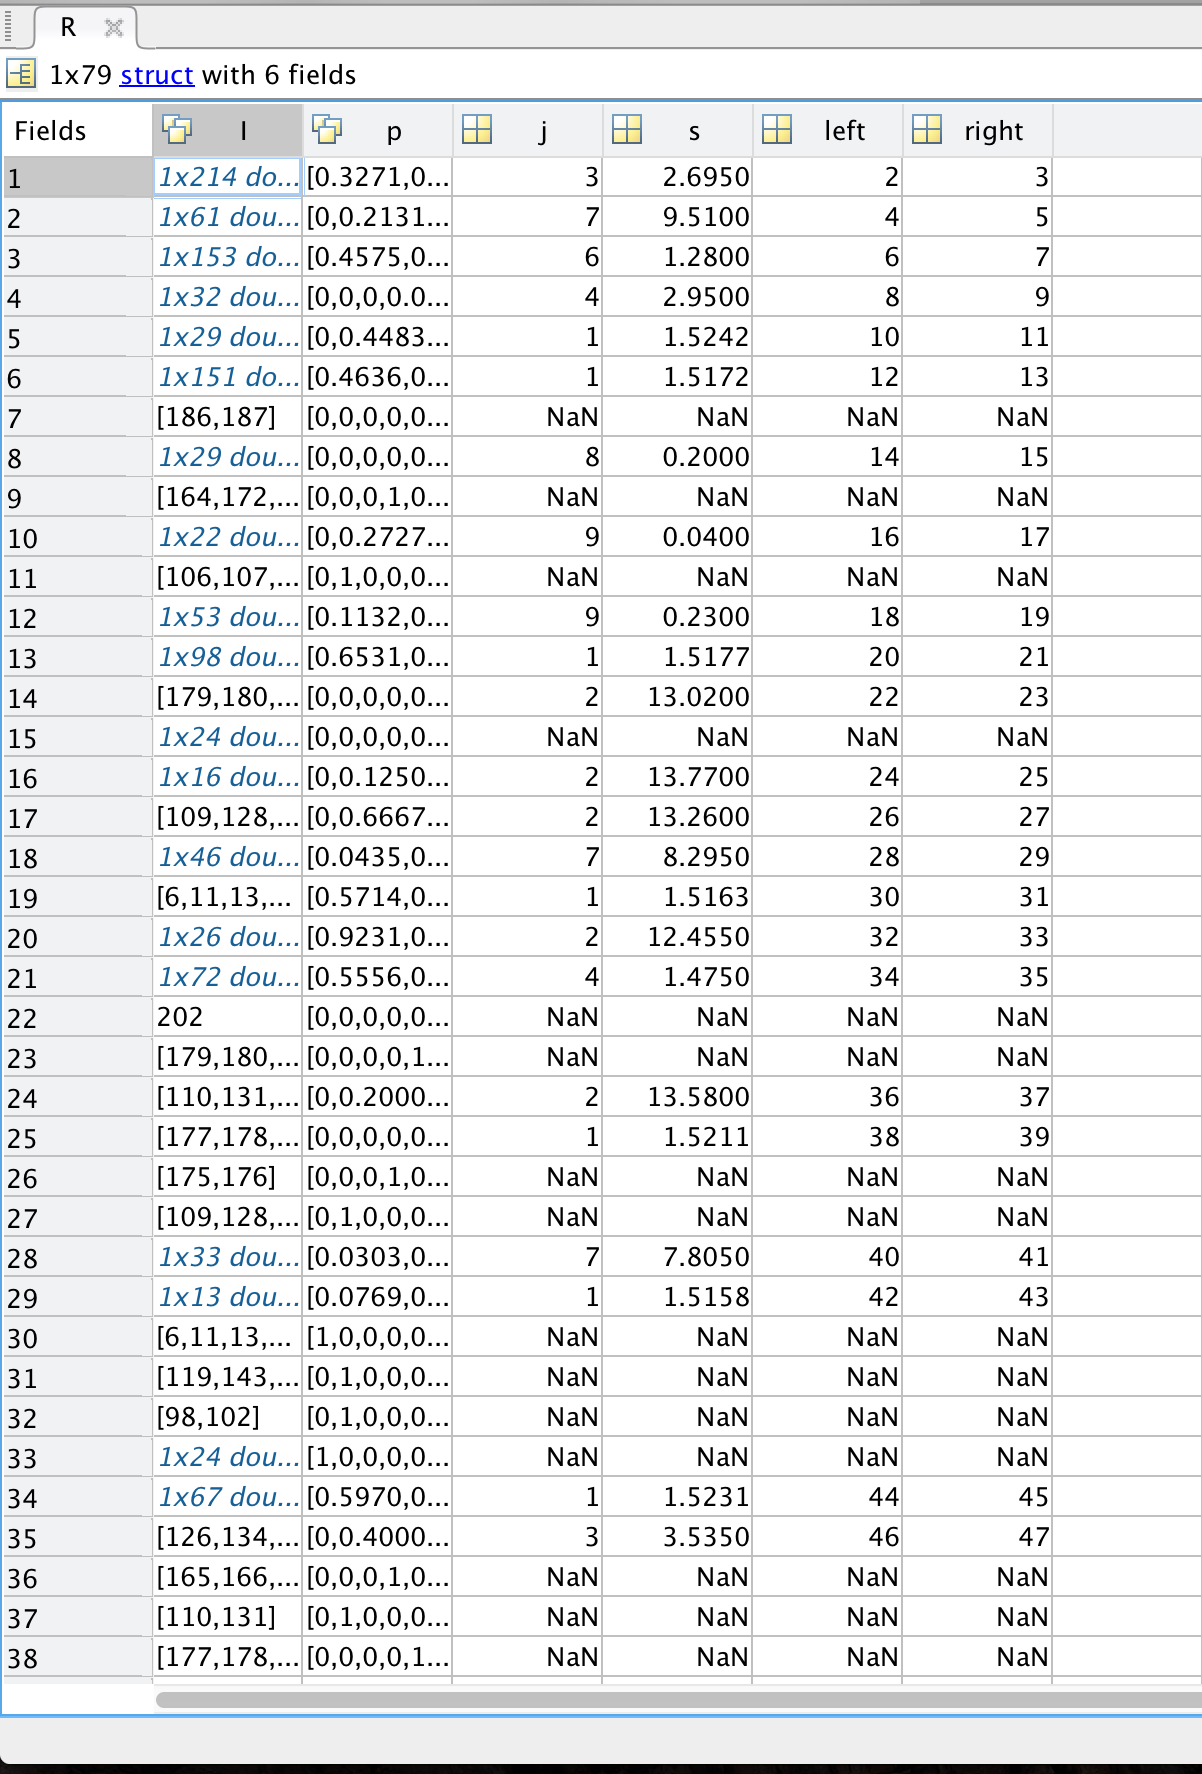
\includegraphics[width=12cm, height=5cm]{GlassData_T_max.png}
    }
    \caption{\label{fig:my figure}The Array R of structs representing all 79 nodes and leaves that define T\_max.  To prove this is in fact T\_max, the sum of all the indices of pure nodes is 214, therefore all data points are captured in a pure node.  We see for instance, that the original node containing all data points can be optimally split in its 3rd dimension by a value 2.695, which will yield its left child at index 2 and right child at index 3. }
\end{figure}


\section*{Pruning the Tree}
\subsection*{Idea}
While for the training set T\_max will perform optimally and properly classify all data points, this tree will often be overfitted and will not capture the more general differences between data points for when new points are to be tested.  Pruning a tree is when we take a node that is not a leaf, delete its children, and make it a leaf.  In our case all leaves were pure and all non-leaf nodes were mixed.  Therefore, in pruning the tree we will no longer be classifying data only with pure rectangles, but instead will look for the optimal nodes, pure and mixed, that classify the data best.  We need a measure to determine the effectiveness of a node of classifying, which we define as the cost-complexity measure of the tree.  \\
The cost-complexity measure seeks a balance between the misclassification error and the complexity of a tree. We define the cost complexity measure as follows:
\[\rho_{\alpha}(T) = \rho(T) + \alpha|T| \]
where $\rho(T)$ is the misclassification error and $\alpha|T|$ is the complexity.  We define
\[ \rho(T) = \sum_{R\epsilon[leaf]} v(R)r(R) \]
such that v(r) is the weight of the leaf relative to the tree:
\[v(r)=n(R)/n(R(1)) \]
and r(R) is the misclassifcation defined previously.
\\Lastly, the complexity |T| is defined as the number of leaves in the tree

We can calculate the difference between the cost complexity of an original tree T and the tree T-T' (where T' is rooted at $\bar{R}$) as follows:
\begin{equation}
\rho_{\alpha}(T-T') - \rho_{\alpha}(T)=  v(\bar{R})r(\bar{R}) + \alpha - \sum_{leaves T'}v(R)r(R) + \alpha|T' 
\end{equation}

\\An optimal tree is one which will minimize the cost-complexity function.  Note the value of $\alpha$ determines the weighting of the complexity versus the error. A small $\alpha$ will favor complex trees as the complexity has low cost, but as $\alpha$ increases, tress will need to be simpler to minimize $\rho_{\alpha}(T) $

\\Our algorithm will begin with T\_max and will iterate through all nodes of T\_max and calculate their $\rho_{\alpha}(T) $ to determine the best node to prune at. This yields a new pruned tree T' and its corresponding $\alpha$ value.  We continue to prune until we arrive at the tree with only the root node included.

\subsection*{Algorithm}
1.  Initialize: Create a cell T to store all the pruned trees, and set T(1)=$T_max$.  \\Set counter k=0
2.  Iterate: Until $T_k = R_0$
\\(a) Compute the genealogy matrix $G^{m,m}$ such that if $G_{i,j}=1$ node j is a descendant of node i.  
\\(b) For all $\bar{R}$ nodes that are not leaves, calculate the critical point $\alpha(\bar{R})$ where pruning tree at $\bar{R}$ has a cost less than the original tree.  We calculate this using eq (1) above.  
\[
\alpha(\bar{R}) =\dfrac{v(\bar{R})r(\bar{R}) - \sum_{leaves T'}v(R)r(R)}{|T'|-1}
\]
We use the MisclassCost() function to find the v(R)r(R) values.  
(c) Prune the tree at the node $\bar{R}_{prune}$ corresponding to the minimum $\alpha$.  \\
To do so, first we find all nodes that are descendants of $\bar{R}_{prune}$ using G
\begin{verbatim}
    children=find(G(ind,:)==1);
\end{verbatim}
Next, starting from the last child down to the first (in order to preserve ordering), we remove each child from the tree
\begin{verbatim}
    R_curr=R_curr([ 1:children(c)-1, children(c)+1:length(R_curr) ]);
\end{verbatim}
Last, we update the children pointers in the remaining nodes because the indices of nodes have changed following the deletions of leaves.  To do so, we decrement every node's pointer to a child by 1 for every time the pointer is greater than the index of one of $\bar{R}_{prune}$'s children
\\
\\
(d) Increment k and proceed

\section*{Results}
We now have a collect of pruned trees stored in T.  Which pruning is ideal depends on the test set, so we will calculate the specificity for all pruned trees and find the best.   I will examine the results for the 'IrisData.mat' set and the 'GlassData.mat' set.  

\subsection*{Iris Data}
I trained the data with the first 25 points of each class and tested with the remaining 25 of each class (75 points per test).  Using this set, I grew the tree to T\_max as described above.  The tree T\_max can be seen in figure (3)
\begin{figure}[H]
    \centerline
    {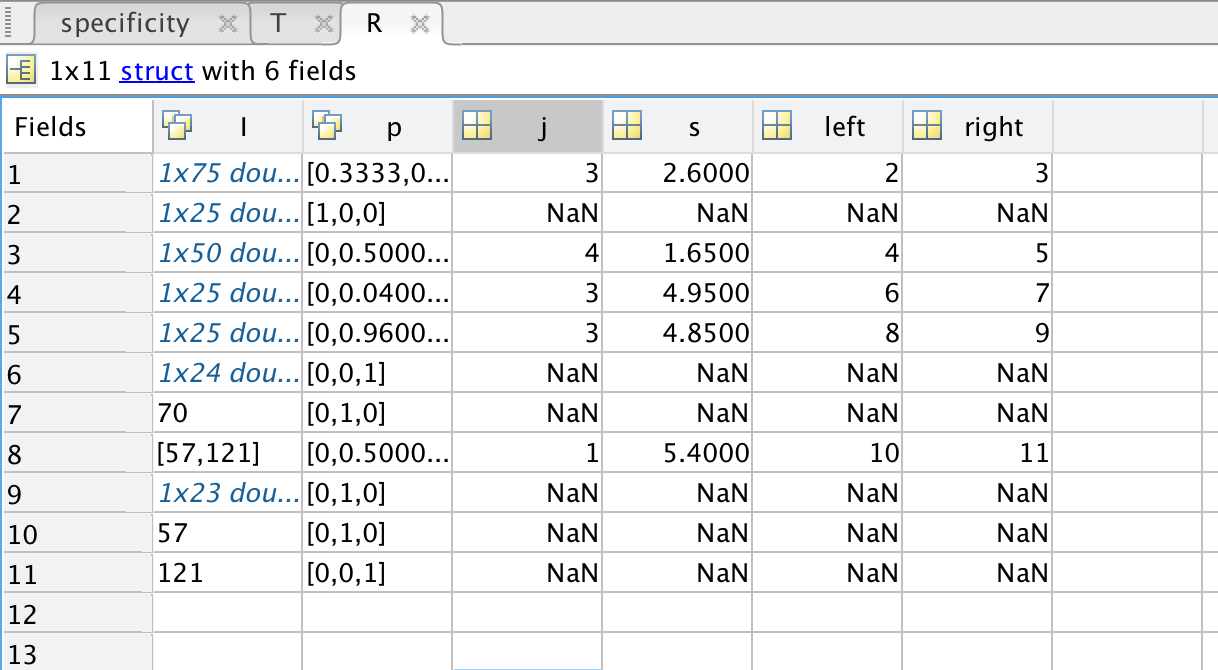
\includegraphics[width=12cm, height=5cm]{IrisData_T_max.png}
    }
    \caption{\label{fig:my figure}The Array R of structs representing all 11 nodes (rectangles) of T\_max.  We see that we quickly distinguished all of class one in the first split, yielding the pure node 2, and mixed node 3, and the remainding splits tried to separate class 2 from 3.  We can separate 96\% pure classes in one more split, and spend the remaining 2 splits separating the one fringe point. }
\end{figure}

Next, I calculated the optimal pruning points to yield 5 increasingly pruned trees, shown in figure (4).  
\begin{figure}[H]
    \centerline
    {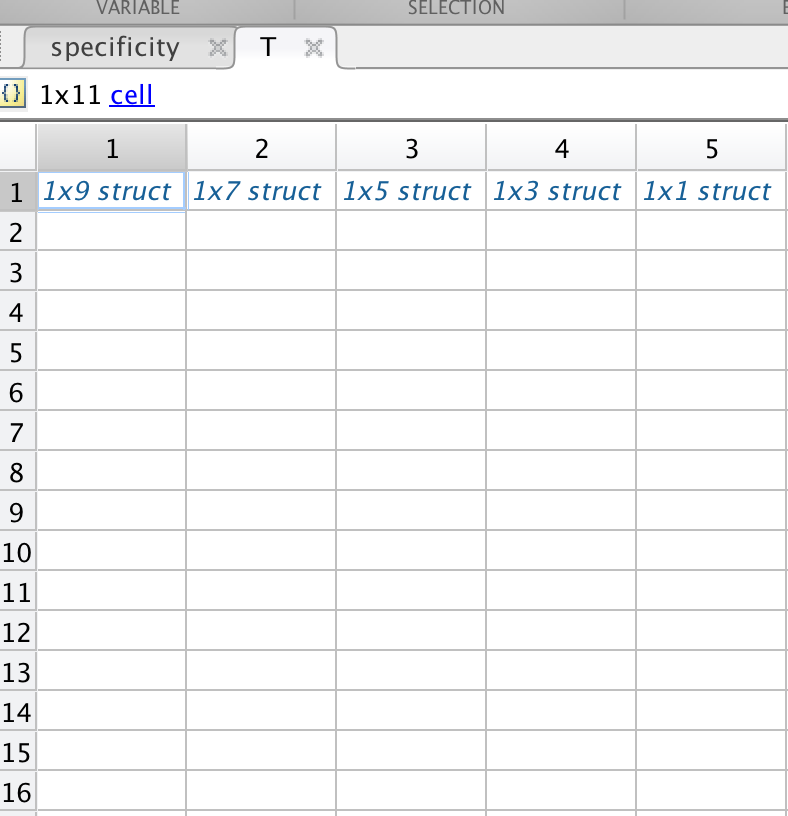
\includegraphics[width=12cm, height=3cm]{IrisData_T.png}
    }
    \caption{\label{fig:my figure} The Matlab references to the increasingly more pruned trees that began at T\_max.  T\_max pruned two children to obtain T{1}, which continued to prune until we arrive at the tree with just the root node.  The optimal tree to classify with depends on the data as we explore below.  }
\end{figure}

The incoming data set determines which tree is best to classify with, so you must test on all trees.  Below are the specificity values for the remaining iris data points classified by each tree. 
\begin{figure}[H]
    \centerline
    {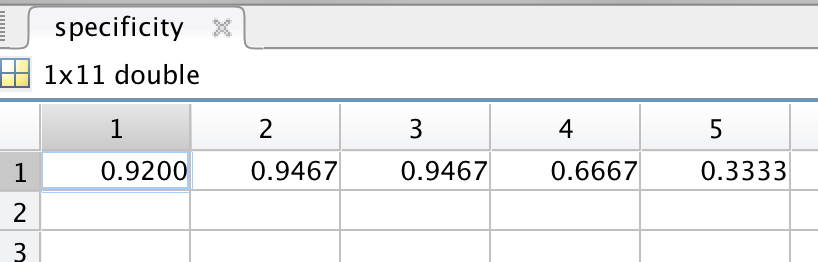
\includegraphics[width=12cm, height=3cm]{IrisData_specificity.png}
    }
    \caption{\label{fig:my figure}The specificity values for the iris data testset classified with each tree T[1:5].  Pruning at trees 1,2, or 3 proves highly effective with specificity values above 90\%.  Trees 4 and 5 represent highly pruned trees with T{5} only being the root node, so it is clear that these would not be effective classifiers.   }
\end{figure}

\subsection*{Glass Data}
I trained the Glass Data with $I_{train}$=[1:35, 71:108, 147:155, 164:170, 177:181, 186:200 ] and tested with $I_{test}$=[36:70, 109:146, 156:163, 170:176, 181:185, 200:214].
\\First we observe $T_{max}$ in figure (6).
\begin{figure}[H]
    \centerline
    {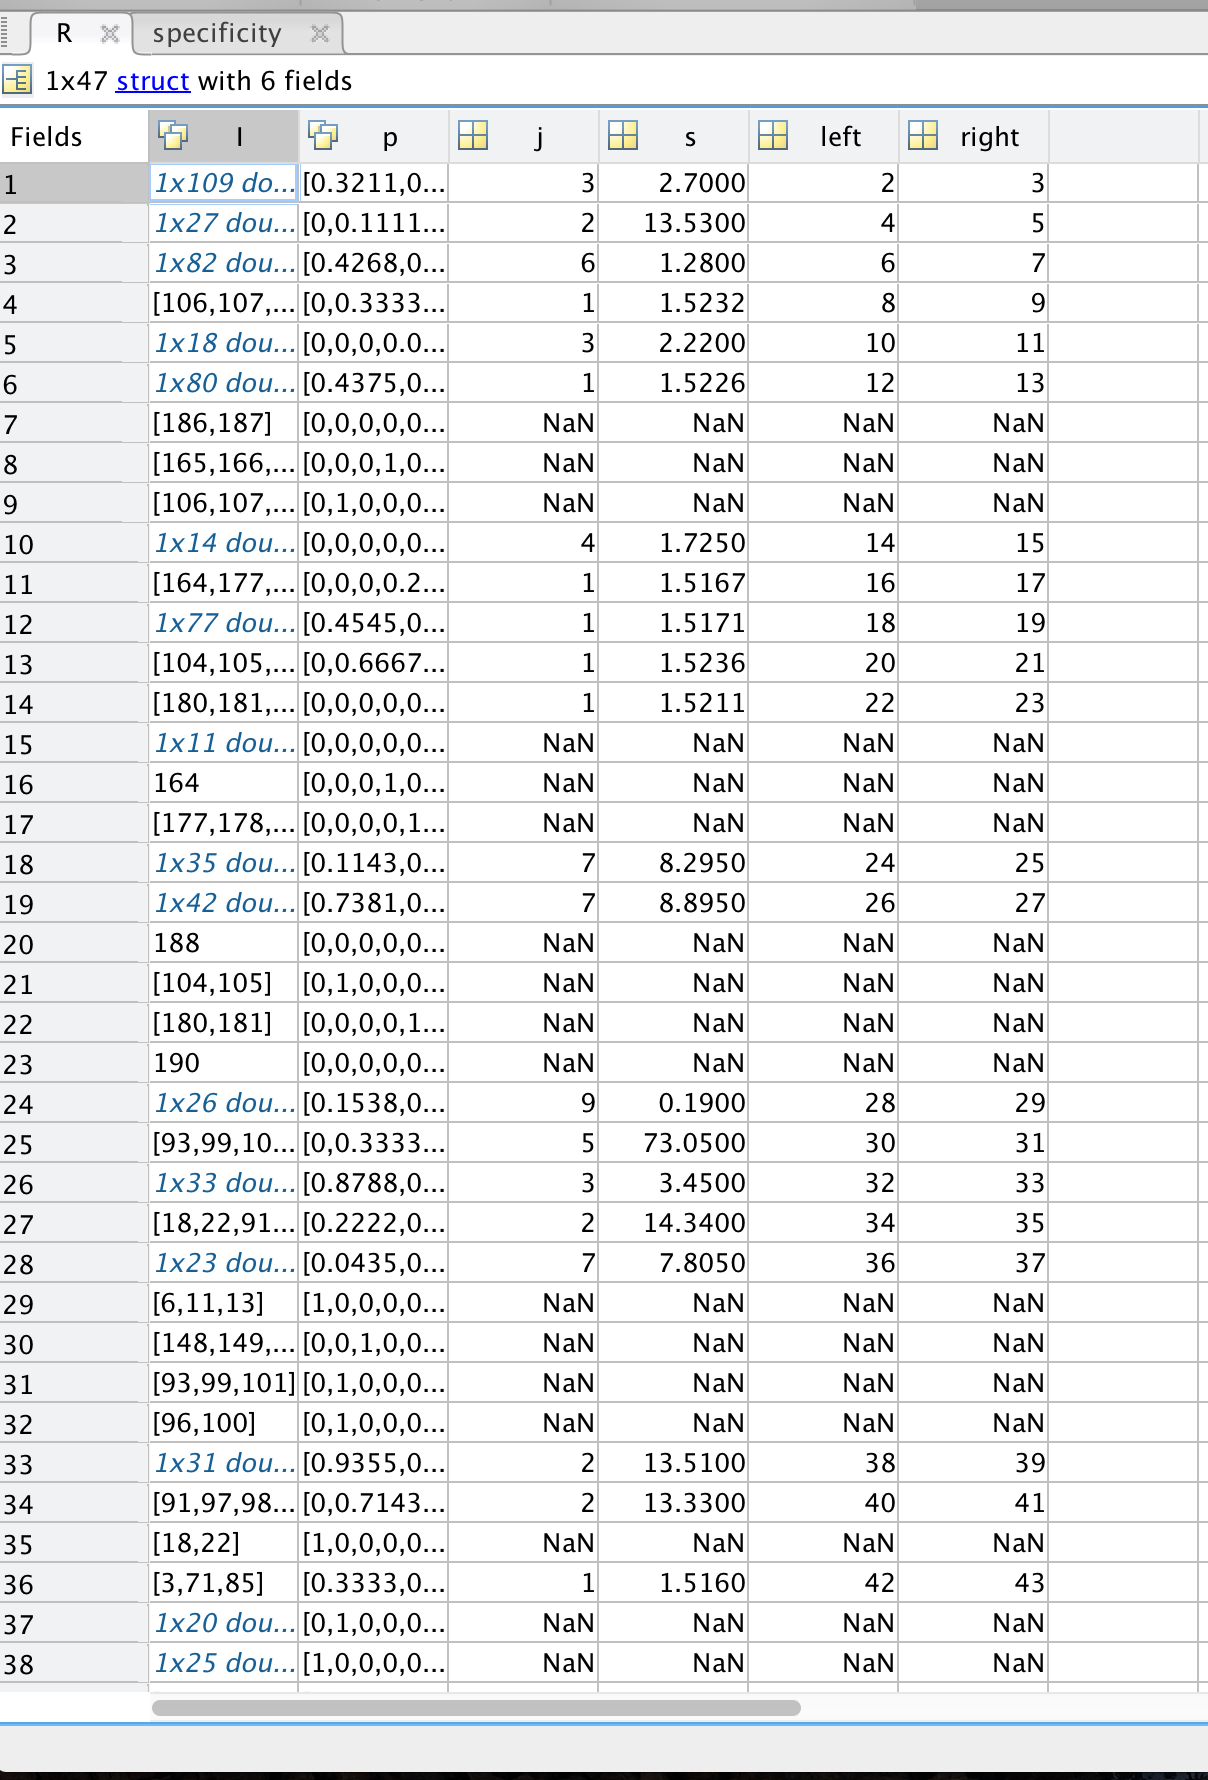
\includegraphics[width=12cm, height=5cm]{GlassData_test_max.png}
    }
    \caption{\label{fig:my figure}The Array R of structs representing all 47 nodes (rectangles) of T\_max for the glass data set. Note that when we trained with the entire test set, there were 79 nodes, but since the data is simpler, so is T\_max.   }
\end{figure}

Next, I pruned the tree, yielding 22 trees of decreasing size.  I tested each tree using the $I_{test}$ set and obtained the following specificity:

 \begin{figure}[H]
    \centerline
    {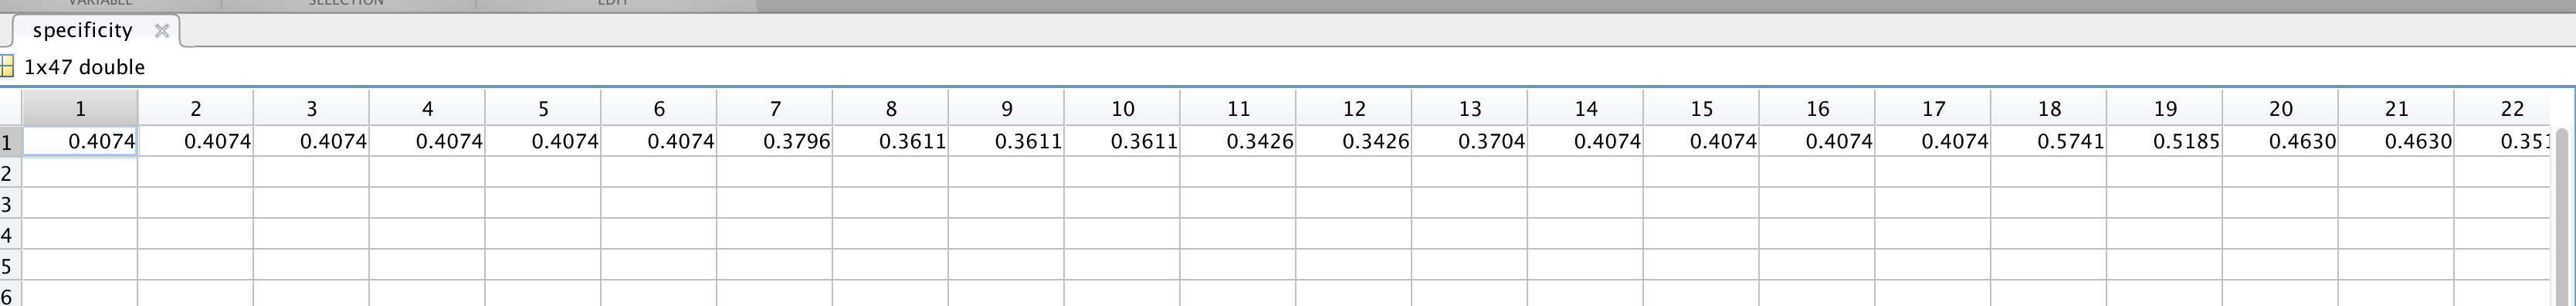
\includegraphics[width=12cm, height=3cm]{GlassData_specificity.png}
    }
    \caption{\label{fig:my figure}The specificity values for the glass data testset classified with each tree T[1:22]. We see that the glass data trees performered far worse with values typically between 40\% and 50\%.  I believe this to be a fault of the data due to the high performance of the iris set.   }
\end{figure}


\end{document}
